% kshadow_natphys.tex -- amsart manuscript.
% Every number is a macro from numbers.tex, generated by
% ../make_paper_numbers.py from ../results/*.json.  Build:
%     cd paper && latexmk -pdf kshadow_natphys.tex
\documentclass[11pt]{amsart}
\usepackage[margin=1in]{geometry}
\usepackage{amssymb,amsthm,mathtools}
\usepackage{graphicx}
\usepackage{booktabs}
\usepackage[hidelinks]{hyperref}
\usepackage{microtype}
\graphicspath{{../figures/}}

%% generated by make_paper_numbers.py from results/*.json; do not edit
\newcommand{\nRec}{153}
\newcommand{\nTone}{111}
\newcommand{\nTtwo}{42}
\newcommand{\thetaOne}{16.0}
\newcommand{\thetaTwo}{23.0}
\newcommand{\thetaThree}{25.3}
\newcommand{\nWithFail}{99}
\newcommand{\failMedian}{4}
\newcommand{\failMax}{31}
\newcommand{\failNone}{12}
\newcommand{\PoneP}{0.068}
\newcommand{\PoneMCratio}{3.0}
\newcommand{\PoneMCp}{1.0\times 10^{-4}}
\newcommand{\PoneMCn}{10000}
\newcommand{\PonePos}{32}
\newcommand{\PoneNeg}{54}
\newcommand{\PoneMeanObs}{1.05}
\newcommand{\PoneMeanNull}{0.35}
\newcommand{\PoneTwoP}{0.34}
\newcommand{\SoneP}{4.1\times 10^{-7}}
\newcommand{\SoneObs}{1455}
\newcommand{\SoneNull}{1134}
\newcommand{\SoneTwoP}{0.004}
\newcommand{\qcPassLost}{6}
\newcommand{\qcFailIntact}{6}
\newcommand{\qcPassIntact}{62}
\newcommand{\qcFailLost}{37}
\newcommand{\hetChi}{367}
\newcommand{\hetNull}{49}
\newcommand{\hetRho}{0.82}
\newcommand{\maxRateName}{P9}
\newcommand{\maxRate}{41}
\newcommand{\recJac}{0.100}
\newcommand{\recNull}{0.057}
\newcommand{\recP}{1.0\times 10^{-3}}
\newcommand{\certExact}{153}
\newcommand{\certRaster}{140}
\newcommand{\stressSets}{1000}
\newcommand{\stressAgree}{1000}
\newcommand{\holesObs}{0.24}
\newcommand{\holesNull}{0.68}
\newcommand{\holesP}{3.4\times 10^{-8}}
\newcommand{\reachNinetyFiveObs}{46.0}
\newcommand{\reachNinetyFiveNull}{30.9}
\newcommand{\reachNinetyFiveNullLo}{28.1}
\newcommand{\reachNinetyFiveNullHi}{33.6}
\newcommand{\reachNinetyObs}{37.6}
\newcommand{\reachNinetyNull}{27.3}
\newcommand{\reachP}{0.003}
\newcommand{\DoneTwo}{19.8}
\newcommand{\DzeroTwo}{23.0}
\newcommand{\DoneP}{1.00}
\newcommand{\DoneBetter}{17}
\newcommand{\DoneWorse}{34}
\newcommand{\DtwoPa}{0.34}
\newcommand{\DtwoPb}{0.90}
\newcommand{\patchArea}{3777}
\newcommand{\gridUnseen}{2082}
\newcommand{\gridUnseenPct}{55.1}
\newcommand{\gridBetti}{(9, 2)}
\newcommand{\greedyUnseen}{1.0}
\newcommand{\greedyBetti}{(1, 1)}
\newcommand{\crownFloor}{12.22}
\newcommand{\crownVerts}{3016}
\newcommand{\minNEight}{66}
\newcommand{\minNTen}{46}
\newcommand{\minNTwelve}{30}
\newcommand{\minNFourteen}{22}
\newcommand{\packEight}{16}
\newcommand{\packTen}{12}
\newcommand{\packFourteen}{8}
\newcommand{\twoAUncov}{1.7}
\newcommand{\twoADisk}{1673}
\newcommand{\twoAFaces}{19396}
\newcommand{\twoBUncov}{0.0}
\newcommand{\twoBDisk}{961}
\newcommand{\twoBFaces}{16835}
\newcommand{\twoBShadow}{(1, 0)}
\newcommand{\twoBMesh}{(1, 1)}
\newcommand{\sigRec}{152}
\newcommand{\sigRows}{8673}
\newcommand{\sigMedianR}{0.886}
\newcommand{\sigRecTwo}{41}
\newcommand{\sigPCh}{64}
\newcommand{\sigPRho}{0.198}
\newcommand{\sigPPos}{64}
\newcommand{\sigPNeg}{0}
\newcommand{\sigPP}{1.8\times 10^{-12}}
\newcommand{\sigSoneCh}{64}
\newcommand{\sigSoneRho}{-0.158}
\newcommand{\sigSonePos}{2}
\newcommand{\sigSoneNeg}{62}
\newcommand{\sigSoneP}{6.0\times 10^{-12}}
\newcommand{\sigSthreeCh}{64}
\newcommand{\sigSthreeRho}{0.294}
\newcommand{\sigSthreePos}{60}
\newcommand{\sigSthreeNeg}{4}
\newcommand{\sigSthreeP}{3.3\times 10^{-12}}
\newcommand{\sigStwoRec}{111}
\newcommand{\sigStwoRho}{0.092}
\newcommand{\sigStwoPos}{75}
\newcommand{\sigStwoP}{7.7\times 10^{-7}}
\newcommand{\topoGainBound}{0.006}
\newcommand{\siteGain}{0.14}
\newcommand{\lamDev}{0.0022}
\newcommand{\xwLamRho}{0.198}
\newcommand{\xwLamP}{1.8\times 10^{-12}}
\newcommand{\xwLamCh}{64}
\newcommand{\xwLamPos}{64}
\newcommand{\xwDoneRho}{0.125}
\newcommand{\xwDoneP}{8.3\times 10^{-7}}
\newcommand{\xwDoneCh}{24}
\newcommand{\xwDonePos}{21}
\newcommand{\xwDthreeRho}{0.169}
\newcommand{\xwDthreeP}{2.8\times 10^{-12}}
\newcommand{\xwDthreeCh}{63}
\newcommand{\xwDthreePos}{62}
\newcommand{\xwNtwoRho}{0.184}
\newcommand{\xwNtwoP}{1.8\times 10^{-12}}
\newcommand{\xwNtwoCh}{64}
\newcommand{\xwNtwoPos}{64}
\newcommand{\xwPiRho}{0.158}
\newcommand{\xwPiP}{6.0\times 10^{-12}}
\newcommand{\xwPiCh}{64}
\newcommand{\xwPiPos}{62}
\newcommand{\xwLamGivenDoneRho}{0.178}
\newcommand{\xwLamGivenDoneP}{1.8\times 10^{-12}}
\newcommand{\xwLamGivenDoneCh}{64}
\newcommand{\xwLamGivenDonePos}{63}
\newcommand{\xwLamGivenDthreeRho}{0.101}
\newcommand{\xwLamGivenDthreeP}{2.3\times 10^{-10}}
\newcommand{\xwLamGivenDthreeCh}{64}
\newcommand{\xwLamGivenDthreePos}{57}
\newcommand{\xwLamGivenNgoodRho}{0.126}
\newcommand{\xwLamGivenNgoodP}{5.3\times 10^{-10}}
\newcommand{\xwLamGivenNgoodCh}{64}
\newcommand{\xwLamGivenNgoodPos}{52}
\newcommand{\xvLamRho}{0.294}
\newcommand{\xvLamP}{3.3\times 10^{-12}}
\newcommand{\xvLamCh}{64}
\newcommand{\xvLamPos}{60}
\newcommand{\xvDoneRho}{0.177}
\newcommand{\xvDoneP}{0.004}
\newcommand{\xvDoneCh}{8}
\newcommand{\xvDonePos}{8}
\newcommand{\xvDthreeRho}{0.221}
\newcommand{\xvDthreeP}{2.8\times 10^{-10}}
\newcommand{\xvDthreeCh}{56}
\newcommand{\xvDthreePos}{51}
\newcommand{\xvNtwoRho}{0.279}
\newcommand{\xvNtwoP}{4.7\times 10^{-12}}
\newcommand{\xvNtwoCh}{64}
\newcommand{\xvNtwoPos}{60}
\newcommand{\xvPiRho}{0.193}
\newcommand{\xvPiP}{1.3\times 10^{-9}}
\newcommand{\xvPiCh}{60}
\newcommand{\xvPiPos}{53}
\newcommand{\xvLamGivenDoneRho}{0.271}
\newcommand{\xvLamGivenDoneP}{6.8\times 10^{-12}}
\newcommand{\xvLamGivenDoneCh}{64}
\newcommand{\xvLamGivenDonePos}{59}
\newcommand{\xvLamGivenDthreeRho}{0.223}
\newcommand{\xvLamGivenDthreeP}{1.5\times 10^{-10}}
\newcommand{\xvLamGivenDthreeCh}{64}
\newcommand{\xvLamGivenDthreePos}{54}
\newcommand{\xvLamGivenNgoodRho}{0.147}
\newcommand{\xvLamGivenNgoodP}{9.0\times 10^{-9}}
\newcommand{\xvLamGivenNgoodCh}{64}
\newcommand{\xvLamGivenNgoodPos}{53}
\newcommand{\xcLamRho}{0.109}
\newcommand{\xcLamP}{3.2\times 10^{-10}}
\newcommand{\xcLamCh}{64}
\newcommand{\xcLamPos}{55}
\newcommand{\xcDoneRho}{0.116}
\newcommand{\xcDoneP}{3.0\times 10^{-7}}
\newcommand{\xcDoneCh}{24}
\newcommand{\xcDonePos}{22}
\newcommand{\xcDthreeRho}{0.151}
\newcommand{\xcDthreeP}{2.4\times 10^{-11}}
\newcommand{\xcDthreeCh}{63}
\newcommand{\xcDthreePos}{59}
\newcommand{\xcNtwoRho}{0.098}
\newcommand{\xcNtwoP}{2.6\times 10^{-8}}
\newcommand{\xcNtwoCh}{64}
\newcommand{\xcNtwoPos}{53}
\newcommand{\xcPiRho}{0.144}
\newcommand{\xcPiP}{4.8\times 10^{-11}}
\newcommand{\xcPiCh}{64}
\newcommand{\xcPiPos}{57}
\newcommand{\xcLamGivenDoneRho}{0.092}
\newcommand{\xcLamGivenDoneP}{1.2\times 10^{-7}}
\newcommand{\xcLamGivenDoneCh}{64}
\newcommand{\xcLamGivenDonePos}{50}
\newcommand{\xcLamGivenDthreeRho}{0.052}
\newcommand{\xcLamGivenDthreeP}{0.008}
\newcommand{\xcLamGivenDthreeCh}{64}
\newcommand{\xcLamGivenDthreePos}{39}
\newcommand{\xcLamGivenNgoodRho}{0.139}
\newcommand{\xcLamGivenNgoodP}{1.3\times 10^{-10}}
\newcommand{\xcLamGivenNgoodCh}{64}
\newcommand{\xcLamGivenNgoodPos}{57}
\newcommand{\xdLamRho}{0.161}
\newcommand{\xdLamP}{3.6\times 10^{-9}}
\newcommand{\xdLamCh}{64}
\newcommand{\xdLamPos}{49}
\newcommand{\xdDoneRho}{0.137}
\newcommand{\xdDoneP}{0.004}
\newcommand{\xdDoneCh}{8}
\newcommand{\xdDonePos}{8}
\newcommand{\xdDthreeRho}{0.167}
\newcommand{\xdDthreeP}{9.7\times 10^{-8}}
\newcommand{\xdDthreeCh}{56}
\newcommand{\xdDthreePos}{46}
\newcommand{\xdNtwoRho}{0.153}
\newcommand{\xdNtwoP}{9.1\times 10^{-8}}
\newcommand{\xdNtwoCh}{64}
\newcommand{\xdNtwoPos}{48}
\newcommand{\xdPiRho}{0.165}
\newcommand{\xdPiP}{1.1\times 10^{-7}}
\newcommand{\xdPiCh}{60}
\newcommand{\xdPiPos}{51}
\newcommand{\xdLamGivenDoneRho}{0.162}
\newcommand{\xdLamGivenDoneP}{2.8\times 10^{-8}}
\newcommand{\xdLamGivenDoneCh}{64}
\newcommand{\xdLamGivenDonePos}{48}
\newcommand{\xdLamGivenDthreeRho}{0.073}
\newcommand{\xdLamGivenDthreeP}{1.9\times 10^{-4}}
\newcommand{\xdLamGivenDthreeCh}{64}
\newcommand{\xdLamGivenDthreePos}{42}
\newcommand{\xdLamGivenNgoodRho}{0.179}
\newcommand{\xdLamGivenNgoodP}{5.6\times 10^{-10}}
\newcommand{\xdLamGivenNgoodCh}{64}
\newcommand{\xdLamGivenNgoodPos}{55}
\newcommand{\cvzMone}{0.027}
\newcommand{\tezMone}{0.033}
\newcommand{\cvzMtwo}{0.051}
\newcommand{\tezMtwo}{0.058}
\newcommand{\cvzMthree}{0.049}
\newcommand{\tezMthree}{0.062}
\newcommand{\cvzMfour}{0.050}
\newcommand{\tezMfour}{0.063}
\newcommand{\cvzMfive}{0.192}
\newcommand{\tezMfive}{0.222}
\newcommand{\cvzMsix}{0.192}
\newcommand{\tezMsix}{0.226}
\newcommand{\cveMone}{0.041}
\newcommand{\teeMone}{0.044}
\newcommand{\cveMtwo}{0.100}
\newcommand{\teeMtwo}{0.101}
\newcommand{\cveMthree}{0.099}
\newcommand{\teeMthree}{0.105}
\newcommand{\cveMfour}{0.100}
\newcommand{\teeMfour}{0.107}
\newcommand{\cveMfive}{0.207}
\newcommand{\teeMfive}{0.253}
\newcommand{\cveMsix}{0.207}
\newcommand{\teeMsix}{0.258}
\newcommand{\mgAOneObs}{1455}
\newcommand{\mgAOneMargMean}{1114}
\newcommand{\mgAOneMargLo}{1074}
\newcommand{\mgAOneMargHi}{1154}
\newcommand{\mgAOneMargP}{1.0\times 10^{-3}}
\newcommand{\mgAOneUnifMean}{1133}
\newcommand{\mgAOneUnifLo}{1085}
\newcommand{\mgAOneUnifHi}{1184}
\newcommand{\mgAOneUnifP}{1.0\times 10^{-3}}
\newcommand{\mgUOneObs}{1.05}
\newcommand{\mgUOneMargMean}{0.25}
\newcommand{\mgUOneMargLo}{0.16}
\newcommand{\mgUOneMargHi}{0.35}
\newcommand{\mgUOneMargP}{1.0\times 10^{-3}}
\newcommand{\mgUOneUnifMean}{0.35}
\newcommand{\mgUOneUnifLo}{0.24}
\newcommand{\mgUOneUnifHi}{0.47}
\newcommand{\mgUOneUnifP}{1.0\times 10^{-3}}
\newcommand{\mgReachOneObs}{46.0}
\newcommand{\mgReachOneMargMean}{30.7}
\newcommand{\mgReachOneMargLo}{28.3}
\newcommand{\mgReachOneMargHi}{33.5}
\newcommand{\mgReachOneMargP}{1.0\times 10^{-3}}
\newcommand{\mgReachOneUnifMean}{30.8}
\newcommand{\mgReachOneUnifLo}{27.8}
\newcommand{\mgReachOneUnifHi}{33.6}
\newcommand{\mgReachOneUnifP}{1.0\times 10^{-3}}
\newcommand{\mgATwoObs}{510}
\newcommand{\mgATwoMargMean}{369}
\newcommand{\mgATwoMargLo}{349}
\newcommand{\mgATwoMargHi}{393}
\newcommand{\mgATwoMargP}{1.0\times 10^{-3}}
\newcommand{\mgATwoUnifMean}{370}
\newcommand{\mgATwoUnifLo}{344}
\newcommand{\mgATwoUnifHi}{399}
\newcommand{\mgATwoUnifP}{1.0\times 10^{-3}}
\newcommand{\mgUTwoObs}{1.42}
\newcommand{\mgUTwoMargMean}{0.32}
\newcommand{\mgUTwoMargLo}{0.17}
\newcommand{\mgUTwoMargHi}{0.51}
\newcommand{\mgUTwoMargP}{1.0\times 10^{-3}}
\newcommand{\mgUTwoUnifMean}{0.39}
\newcommand{\mgUTwoUnifLo}{0.20}
\newcommand{\mgUTwoUnifHi}{0.62}
\newcommand{\mgUTwoUnifP}{1.0\times 10^{-3}}
\newcommand{\mgReachTwoObs}{54.0}
\newcommand{\mgReachTwoMargMean}{28.6}
\newcommand{\mgReachTwoMargLo}{25.2}
\newcommand{\mgReachTwoMargHi}{34.4}
\newcommand{\mgReachTwoMargP}{1.0\times 10^{-3}}
\newcommand{\mgReachTwoUnifMean}{28.8}
\newcommand{\mgReachTwoUnifLo}{25.8}
\newcommand{\mgReachTwoUnifHi}{34.3}
\newcommand{\mgReachTwoUnifP}{1.0\times 10^{-3}}
\newcommand{\mgNull}{1000}
\newcommand{\mgPfloor}{0.001}
\newcommand{\gBinLo}{10}
\newcommand{\gBinHi}{20}
\newcommand{\gFirstOne}{1.72}
\newcommand{\gSecondOne}{1.34}
\newcommand{\gThirdOne}{1.29}
\newcommand{\xiOne}{36}
\newcommand{\xiOneLo}{20}
\newcommand{\xiOneHi}{45}
\newcommand{\gFirstTwo}{1.84}
\newcommand{\gSecondTwo}{1.51}
\newcommand{\gThirdTwo}{1.29}
\newcommand{\xiTwo}{34}
\newcommand{\xiTwoLo}{17}
\newcommand{\xiTwoHi}{91}
\newcommand{\gNullHiFirst}{1.10}
\newcommand{\nnSpacing}{18}


\newtheorem{theorem}{Theorem}
\newtheorem{proposition}[theorem]{Proposition}
\newtheorem{corollary}[theorem]{Corollary}
\theoremstyle{definition}
\newtheorem{definition}[theorem]{Definition}
\theoremstyle{remark}
\newtheorem{remark}[theorem]{Remark}

\newcommand{\R}{\mathbb{R}}
\newcommand{\Sph}{\mathbb{S}}
\DeclareMathOperator{\area}{area}

\title[Redundant coverage under real contact failure]%
{Redundant coverage of electrode arrays under real contact failure:\\
a topological certificate, and what it does not predict}

\author{Aditi Bose}
\address{Centre for Computational Natural Sciences and Bioinformatics,
International Institute of Information Technology, Hyderabad, India}
\urladdr{https://orcid.org/0000-0002-3036-8223}

\author{Deep Bhattacharjee}
\address{[affiliation to be supplied by the author]}
\urladdr{https://orcid.org/0000-0003-0466-750X}

\author{Ushashi Bhattacharya}
\address{[affiliation to be supplied by the author]}
\urladdr{https://orcid.org/0009-0002-2254-3914}

\date{\today}

\begin{document}

\begin{abstract}
Electrode arrays lose contacts, so the region an array can be trusted to
record is the region its contacts see at least $k$ times, not the area they
see once. We compute the topology of that region from which contact
footprints overlap, by Sheehy's multicover nerve theorem, and test it on the
channel failures marked by data curators in \nRec{} recordings from a
64-channel EEG cap. On every real failure pattern, the certificate equals the
exact topology of the $k$-fold region. Real failures are not random. Failed
channels are neighbours more often than chance, failure sets recur within a
subject, and a minority of recordings lose far more of the target than random
failures would take, although the pre-specified primary test of uncovered
area did not reach significance ($p=\PoneP$). The clustering survives a null that keeps every channel's own failure rate,
and neighbouring channels fail together over a correlation length of about
\xiOne$^\circ$. Under a plan
fixed before any signal was loaded, the redundancy left around a channel
predicted how well its signal could be rebuilt from the other channels. All
four pre-specified tests agreed, and the effect survives removing
recording-level effects. But redundancy depth is a sum of pairwise distance
terms, and out of sample the topology of the surviving coverage changed the
explained variance by at most \topoGainBound{} beyond the distances to the
nearest survivors. An array optimised for double coverage did not survive the
real failures better than the standard cap. The certificate is exact and
useful for auditing an array. On this evidence, its physical content is
geometric.
\end{abstract}

\maketitle

\section{Introduction}

An electrode array on the scalp or the cortex is judged by what it sees, and
it keeps being judged after some of its contacts fail. A contact can lose its
seal, pick up line noise, or sit over a region it cannot record from. In the
first sessions of the EEG dataset studied here, the curators discarded a
median of \failMedian{} of 64 channels per recording and up to \failMax{}, and
only \failNone{} of \nTone{} recordings kept all 64. What
matters for an array is therefore not the area its contacts see once, but the
region they see at least $k$ times, and whether that region still contains the
target when $k-1$ of them are gone.

This paper asks three questions of that region, on real data. Can its shape be
certified from which contact footprints overlap, without rasterising
anything? Do real contact failures damage it the way random failures would? And
does redundancy measured this way predict something physical: how well the
signal of a lost channel can be rebuilt from the channels that remain?

The first question has a known answer. For a family of convex footprints, the
region seen at least $k$ times is homotopy equivalent to a simplicial complex
built from the nerve of the family: Sheehy's multicover nerve
theorem~\cite{Sheehy2012}; see also~\cite{EdelsbrunnerOsang2021,CavannaGardnerSheehy2017}
and, for the case $k=1$ and the use of such complexes for sensor coverage,
\cite{Borsuk1948,deSilvaGhrist2007}. We use it as a tool and claim no new
theorem about it. What is new here is empirical: the certificate is run on
the failure patterns of \nRec{} real EEG recordings, where the curators of an
open dataset marked the bad channels~\cite{HatlestadHall2022,ds003775};
its answers are checked against the exact topology of the arrangement of cap
boundaries; and the redundancy it measures is tested, under an analysis plan
fixed before any signal was loaded, against the quality with which each
channel is rebuilt from the others.

The answers are mixed, and we report them as they came out. The certificate
agrees with the exact topology on every real failure pattern. Real failures
are not random: they fall on neighbouring channels, they recur in the same
subject, and a minority of recordings lose far more of the target than random
failures of the same size would take. The clustering is not a gradient in failure rate. It survives a null that
keeps every channel's failure rate, and channels fail together over a
correlation length of about \xiOne$^\circ$.
Under a plan fixed before any signal was loaded, the redundancy that failures
leave around a channel predicts how well that channel's signal is rebuilt
from the others. But the redundancy that predicts is a sum of distance terms
(Proposition~\ref{prop:pairwise}), and out of sample the topology of the
surviving coverage adds nothing measurable to the distances to the nearest
survivors.
An array optimised for tight double coverage did not survive the real
failures better than the standard cap.

\section{The certificate}\label{sec:framework}

Let $X$ be the scalp sphere or the cortical surface with its geodesic metric,
$T\subset X$ the target, and $B_1,\dots,B_n$ the footprints of $n$ contacts,
geodesic balls of a common radius $\theta$ about the contact positions
$c_1,\dots,c_n$. The multiplicity of a point is
$m(x)=\#\{i : x\in B_i\}$ and the $k$-fold region is
$R_k=\{x : m(x)\ge k\}$, so that $R_1\supseteq R_2\supseteq\cdots$.

\begin{definition}
The nerve $N$ of the family is the simplicial complex of index sets $\sigma$
with $\bigcap_{i\in\sigma}B_i\neq\emptyset$. Its $k$-shadow $\Delta_k(N)$ has one
vertex for each face of $N$ with exactly $k$ elements, and a set of such
vertices spans a simplex when the union of their index sets is a face of $N$.
\end{definition}

\begin{theorem}[Sheehy~\cite{Sheehy2012}]\label{thm:multicover}
If every nonempty intersection of footprints is contractible (for instance,
if the footprints are convex), then $\Delta_k(N)$ is homotopy equivalent to
$R_k$ for every $k\ge1$.
\end{theorem}

It is the nerve theorem~\cite{Borsuk1948} applied to the cover of $R_k$ by
the sets $B_\sigma=\bigcap_{i\in\sigma}B_i$ with $|\sigma|=k$: a family of
such sets meets exactly when the union of their index sets is a face of $N$,
so the nerve of that cover is $\Delta_k(N)$, and each of its intersections is
itself an intersection of footprints.

Everything about the shape of $R_k$ can thus be read from which footprints
meet, and for equal balls in the plane, or caps of radius below
$30^\circ$ on the sphere, Helly's theorem~\cite{Helly1923} reduces that to
pairs and triples. We call the \emph{certified level} of an array the largest
$k$ such that $\Delta_j(N)$ has Betti numbers $(b_0,b_1)=(1,0)$ for every
$j\le k$. The condition is not monotone in $k$ and has to be checked at every
level.

The certificate gives the shape of $R_k$, not its position. It neither
proves nor refutes that $R_k$ contains the target. A second component or a
hole can lie outside $T$ while $T\subseteq R_k$, and a disk-like $R_k$ can miss
part of $T$; Section~\ref{sec:cortex} has an example of each. Whether $T$ is
covered is therefore always checked directly here. A combinatorial condition,
checkable on $N$ and a description of $T$, that forces $T\subseteq R_k$ is
open, and is the first of the two problems of Section~\ref{sec:discussion}.

The certificate does give a guarantee that is purely combinatorial.

\begin{proposition}[dropout]\label{prop:dropout}
Under the hypothesis of Theorem~\ref{thm:multicover}, suppose
$\Delta_{q+1}(N)$ is connected and every contact belongs to a face of $N$
with $q+1$ elements. Then for any set $F$ of at most $q$ failed contacts, the
union of the surviving footprints is connected.
\end{proposition}

\begin{proof}
A point of $R_{q+1}$ lies in $q+1$ footprints, at most $q$ of which failed,
so $R_{q+1}\subseteq\bigcup_{i\notin F}B_i$. By Theorem~\ref{thm:multicover}
$R_{q+1}$ is connected. A surviving footprint $B_i$ contains a point of a
$(q+1)$-fold intersection, hence a point of $R_{q+1}$, and is itself
connected. The union of the surviving footprints is $R_{q+1}$ together with
connected sets that each meet it, so it is connected.
\end{proof}

We call the largest such $q$ the \emph{dropout margin}. One more
observation turned out to decide how the signal-level test of
Section~\ref{sec:signal} can be read, so we state it here.

\begin{proposition}[averaged multiplicity is pairwise]\label{prop:pairwise}
Let $\mu$ be the area measure, $c$ a contact, and $S$ a set of other
contacts. The mean multiplicity of the surviving footprints over the
footprint of $c$,
\[
\lambda(c,S)=\frac{1}{\mu(B_c)}\int_{B_c}\sum_{j\in S}\mathbf 1_{B_j}\,d\mu
=\sum_{j\in S}\frac{\mu(B_c\cap B_j)}{\mu(B_c)},
\]
is additive over $S$. On the sphere, with caps of common radius $\theta$, each
term depends only on the angle $\gamma_{cj}$ between $c$ and $j$:
$\lambda(c,S)=\sum_{j\in S}K_\theta(\gamma_{cj})$, where $K_\theta(\gamma)$
is the fraction of a cap covered by a second cap at angle $\gamma$, which
vanishes for $\gamma\ge2\theta$.
\end{proposition}

\begin{proof}
Exchange the finite sum and the integral. On the sphere, the rotation group
acts transitively on pairs of points at a given angle, so
$\mu(B_c\cap B_j)$ depends on $\gamma_{cj}$ alone.
\end{proof}

So $\lambda$, the natural ``redundancy depth'' of a contact, is a kernel sum
over the distances from $c$ to the survivors, one survivor at a time. It
cannot see how the survivors overlap one another, and that overlap is exactly
what the topology of $R_k$ records. The private territory
$\pi(c,S)=\mu(B_c\setminus\bigcup_{j\in S}B_j)/\mu(B_c)$ does depend on it,
through inclusion and exclusion over all orders, and so does every Betti
number. A test in which $\lambda$ predicts a physical quantity is therefore a
test of geometry, however it comes out. Only a quantity that is not additive
over survivors can show that topology does work that distances do not.

\section{Placement on a template cortex}\label{sec:cortex}

On a \patchArea{}\,mm$^2$ patch of the left parietal pial surface of the
colin27 template~\cite{Holmes1998,Oostenveld2011}, with footprints of
geodesic radius 8\,mm, the $8\times8$ grid of the FieldTrip tutorial layout,
transferred to the template, leaves \gridUnseen{}\,mm$^2$
(\gridUnseenPct\%) of the patch unseen, with $\Delta_1(N)$ of Betti numbers
\gridBetti{}. The same number of contacts placed by farthest-point sampling
in the geodesic metric leaves \greedyUnseen{}\,mm$^2$ unseen, with Betti
numbers \greedyBetti{}, and \minNEight{} contacts leave nothing unseen at
certified level~1 (Fig.~\ref{fig:cortex}). The comparison is between
placements, not devices. The grid was laid out for a larger region, and the
farthest-point design uses any pial vertex, including sulcal depths that a
subdural grid cannot reach. The constraint that binds a real subdural array
is the \emph{crown floor}: with all \crownVerts{} gyral-crown vertices of the
patch as contacts, some point of the patch is still \crownFloor\,mm from
every one of them. So no surface array whose footprint radius is below
\crownFloor\,mm can see the whole patch, however many contacts it has.

Geodesic footprints on a folded surface are not convex, so
Theorem~\ref{thm:multicover} is not guaranteed there, and every certificate
on the cortex was checked against the $k$-fold region computed directly on
the mesh. The check matters. With 112 contacts at 9\,mm, the whole patch is
seen at least twice by direct computation (\twoBUncov\,mm$^2$ seen fewer than
twice), and the certificate gives $\Delta_2(N)$ Betti numbers \twoBShadow{}.
But the mesh finds \twoBMesh{} for $R_2$: a hole outside the patch that the
nerve misses, with \twoBDisk{} of the \twoBFaces{} nerve faces failing the
discrete disk test. With 96 contacts at 10\,mm the two computations agree at
every level and the certified level is~2, yet \twoAUncov\,mm$^2$ of the patch
is seen only once. The certificate is correct there and still does not imply
containment.

\begin{figure}[t]
\centering
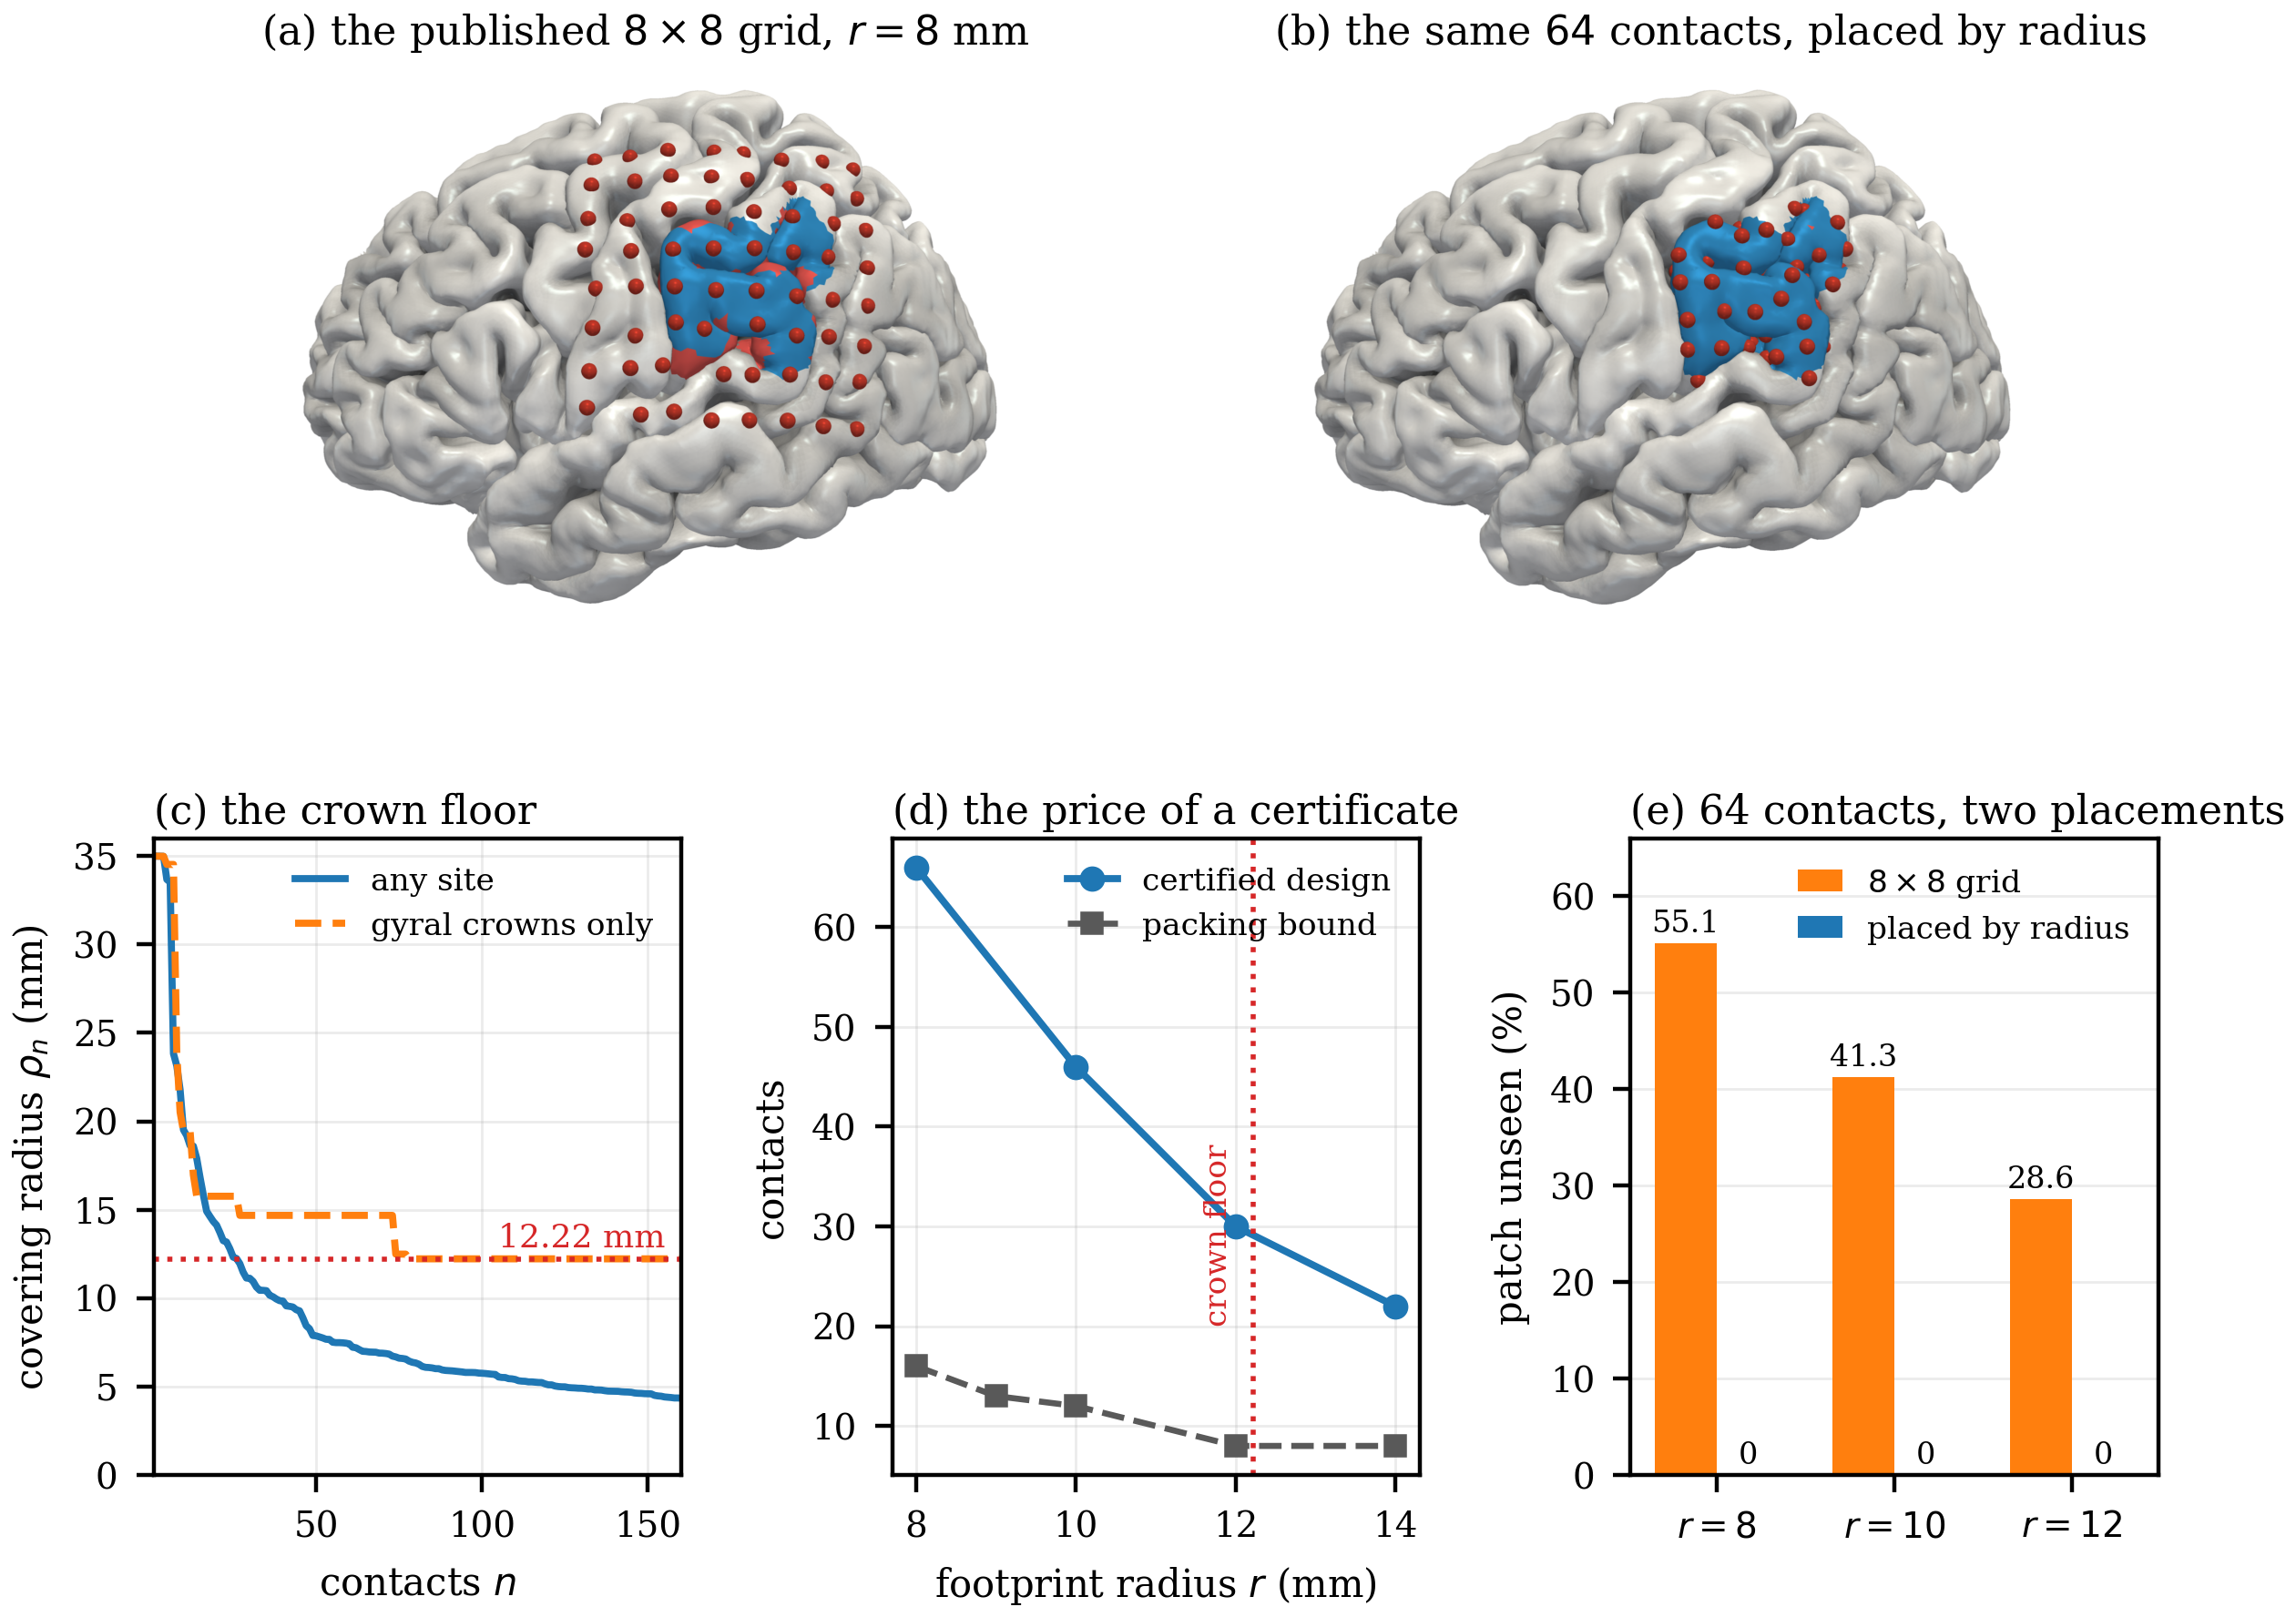
\includegraphics[width=\textwidth]{fig_optimal.png}
\caption{Placement on the colin27 template. (a) The $8\times8$ tutorial grid
and (b) 64 contacts placed by geodesic farthest-point sampling, with the
target patch in blue and 8\,mm footprints. (c) Covering radius against contact
count, for sites anywhere on the patch and for gyral crowns only; the crown
curve cannot fall below \crownFloor\,mm. (d) The smallest contact count with
certified level~1 at each footprint radius, against the packing lower bound.
(e) Patch unseen by the two 64-contact placements.}
\label{fig:cortex}
\end{figure}

\section{Real contact failures}\label{sec:failures}

\subsection*{Data and plan} OpenNeuro ds003775 v1.2.1~\cite{ds003775} holds
resting-state EEG from \nTone{} adults on a 64-channel BioSemi cap, \nTtwo{}
of them recorded again 2--3 months later, with the channels that the
curators' automated pipeline marked bad in each of the \nRec{}
recordings~\cite{HatlestadHall2022}. The data descriptor gives two channel
retention figures, and the failure table rebuilt from the dataset's public
mirror reproduces both exactly. Each channel gets a spherical-cap footprint.
The target $T$ is the scalp inside the Fpz--T7--Oz--T8 circumference, and the
intact cap sees all of $T$ once, twice and three times from cap radii
\thetaOne, \thetaTwo{} and \thetaThree{} degrees. The analysis plan was fixed
before any outcome was computed. It set the primary radius at $23.5^\circ$,
where the intact cap sees $T$ twice, so that no single failure can uncover
any of it; the first sessions as the primary cohort and the second as
replication; and, as the null, each failure set replaced by a uniformly
random set of the same size.

\subsection*{The certificate on real failures}
On all \certExact{} surviving caps the Betti numbers of $\Delta_1$ and
$\Delta_2$, computed from intersection data alone, equal those of the $k$-fold
region computed exactly from the arrangement of boundary circles, and they
agree on \stressAgree{} of \stressSets{} random failure sets. A raster of the
multiplicity function agrees on \certRaster{} of the \certExact{}; in the
others it reports extra components or holes, which is a resolution effect.

\subsection*{Pre-specified tests}
The primary outcome was the uncovered fraction of $T$ after failure. Its
one-sided Wilcoxon signed-rank test against the random expectation, over the
\nWithFail{} first-session recordings with at least one failure, gave
$p=\PoneP$, so the primary test \emph{failed} at $\alpha=0.05$. The plan named
a second test for the same outcome, a Monte Carlo test of the cohort total,
and it gave $p=\PoneMCp$: real failures uncover \PoneMCratio{} times the area
that random failures of the same sizes uncover (mean \PoneMeanObs\% of $T$
against \PoneMeanNull\%). The two disagree because the effect is carried by
a minority of recordings. \PonePos{} recordings lose more than their random
expectation and \PoneNeg{} lose less, but those that lose more lose much
more. Because the plan did not say how to combine the two tests, we
report the primary endpoint as not established.

The secondary tests were clearer. Failed channels are neighbours more often
than random sets of the same size (\SoneObs{} adjacent failed pairs against
\SoneNull{} expected, $p=\SoneP$; replication $p=\SoneTwoP$). Channels fail at
very different rates, from \maxRate\% for \maxRateName{} down to none
(chi-square \hetChi{} against a null mean of \hetNull{}), and the rate rises
towards the rim (Spearman \hetRho{} with colatitude). Failure sets recur within
a subject (mean Jaccard index \recJac{} between sessions against \recNull{}
for random re-pairings, $p=\recP$). The descriptor's quality rule, ``more
than 90\% of channels kept'', disagrees with the coverage outcome in
\qcPassLost{} recordings that pass it and lose target, and \qcFailIntact{}
that fail it and keep all of $T$. Real failures also punch fewer holes into
the surviving coverage than random ones (mean $b_1$ \holesObs{} against
\holesNull{}, $p=\holesP$). Clustered failures take out a region at the edge
instead of scattering gaps through the interior, and that difference is
topological.

\subsection*{Clustering beyond a gradient in failure rate (exploratory)}
The null of the plan draws failures uniformly, but channels do not fail
uniformly. The channels that fail most are rim channels, and they are each
other's neighbours, so a rate gradient alone would produce adjacent failures
and rim losses with no interaction between failures at all. We therefore
compared the real failures with null cohorts that keep each recording's
number of failures \emph{and} each channel's number of failures, sampled by
curveball swaps~\cite{Strona2014}. The clustering survives. There are
\mgAOneObs{} adjacent failed pairs against \mgAOneMargMean{}
(95\% null range \mgAOneMargLo--\mgAOneMargHi). The mean uncovered target is
\mgUOneObs\% against \mgUOneMargMean\% (\mgUOneMargLo--\mgUOneMargHi\%). The
reach needed at 95\% is \mgReachOneObs$^\circ$ against
\mgReachOneMargMean$^\circ$ (\mgReachOneMargLo--\mgReachOneMargHi$^\circ$). In
each case no null cohort of \mgNull{} reached the observed value
($p\le\mgPfloor$), and the second sessions give the same answer. Channels at
\gBinLo--\gBinHi$^\circ$ from each other fail together \gFirstOne{} times as
often as their own rates predict (second sessions \gFirstTwo; the 95\% null
range reaches \gNullHiFirst). The excess falls to $1/e$ of that by
$\xi\approx\xiOne^\circ$ (bootstrap 95\% interval \xiOneLo--\xiOneHi$^\circ$;
second sessions \xiTwo$^\circ$, \xiTwoLo--\xiTwoHi$^\circ$), about two
inter-electrode spacings of \nnSpacing$^\circ$ (Fig.~\ref{fig:signal}c). Failure on this cap is a
spatially correlated process with a measurable correlation length. Its source
is not identified here; a shared electrolyte bridge, a cap that sits poorly
over one region, and muscle or movement artefact over the temporal rim are all
candidates.

\subsection*{The reach real failures demand (exploratory)}
For each recording, $\rho_1(S)$ is the smallest cap radius at which the
survivors see all of $T$. Keeping all of $T$ seen in 95\% of first-session
recordings takes \reachNinetyFiveObs$^\circ$, against \reachNinetyFiveNull$^\circ$
(95\% interval \reachNinetyFiveNullLo--\reachNinetyFiveNullHi$^\circ$) for random
failures of the same sizes. At 90\% it takes \reachNinetyObs$^\circ$ against
\reachNinetyNull$^\circ$.

\subsection*{A layout optimised for double coverage (exploratory)}
Minimising the 2-fold covering radius of $T$ over 64 positions brings it from
\DzeroTwo$^\circ$ to \DoneTwo$^\circ$. Carrying the real failures to the new layout by one
assumption (a contact fails where the nearest cap channel failed), the optimised
layout lost more of $T$ than the standard cap in \DoneWorse{} recordings and
less in \DoneBetter{} ($p=\DoneP$ for improvement). Restricting the
optimisation to a colatitude chosen on one half of the subjects and scored on
the other did not help in either fold ($p=\DtwoPa$ and $\DtwoPb$). Tight double
coverage protects against scattered losses, and the real losses are clustered
at the rim.

\begin{figure}[t]
\centering
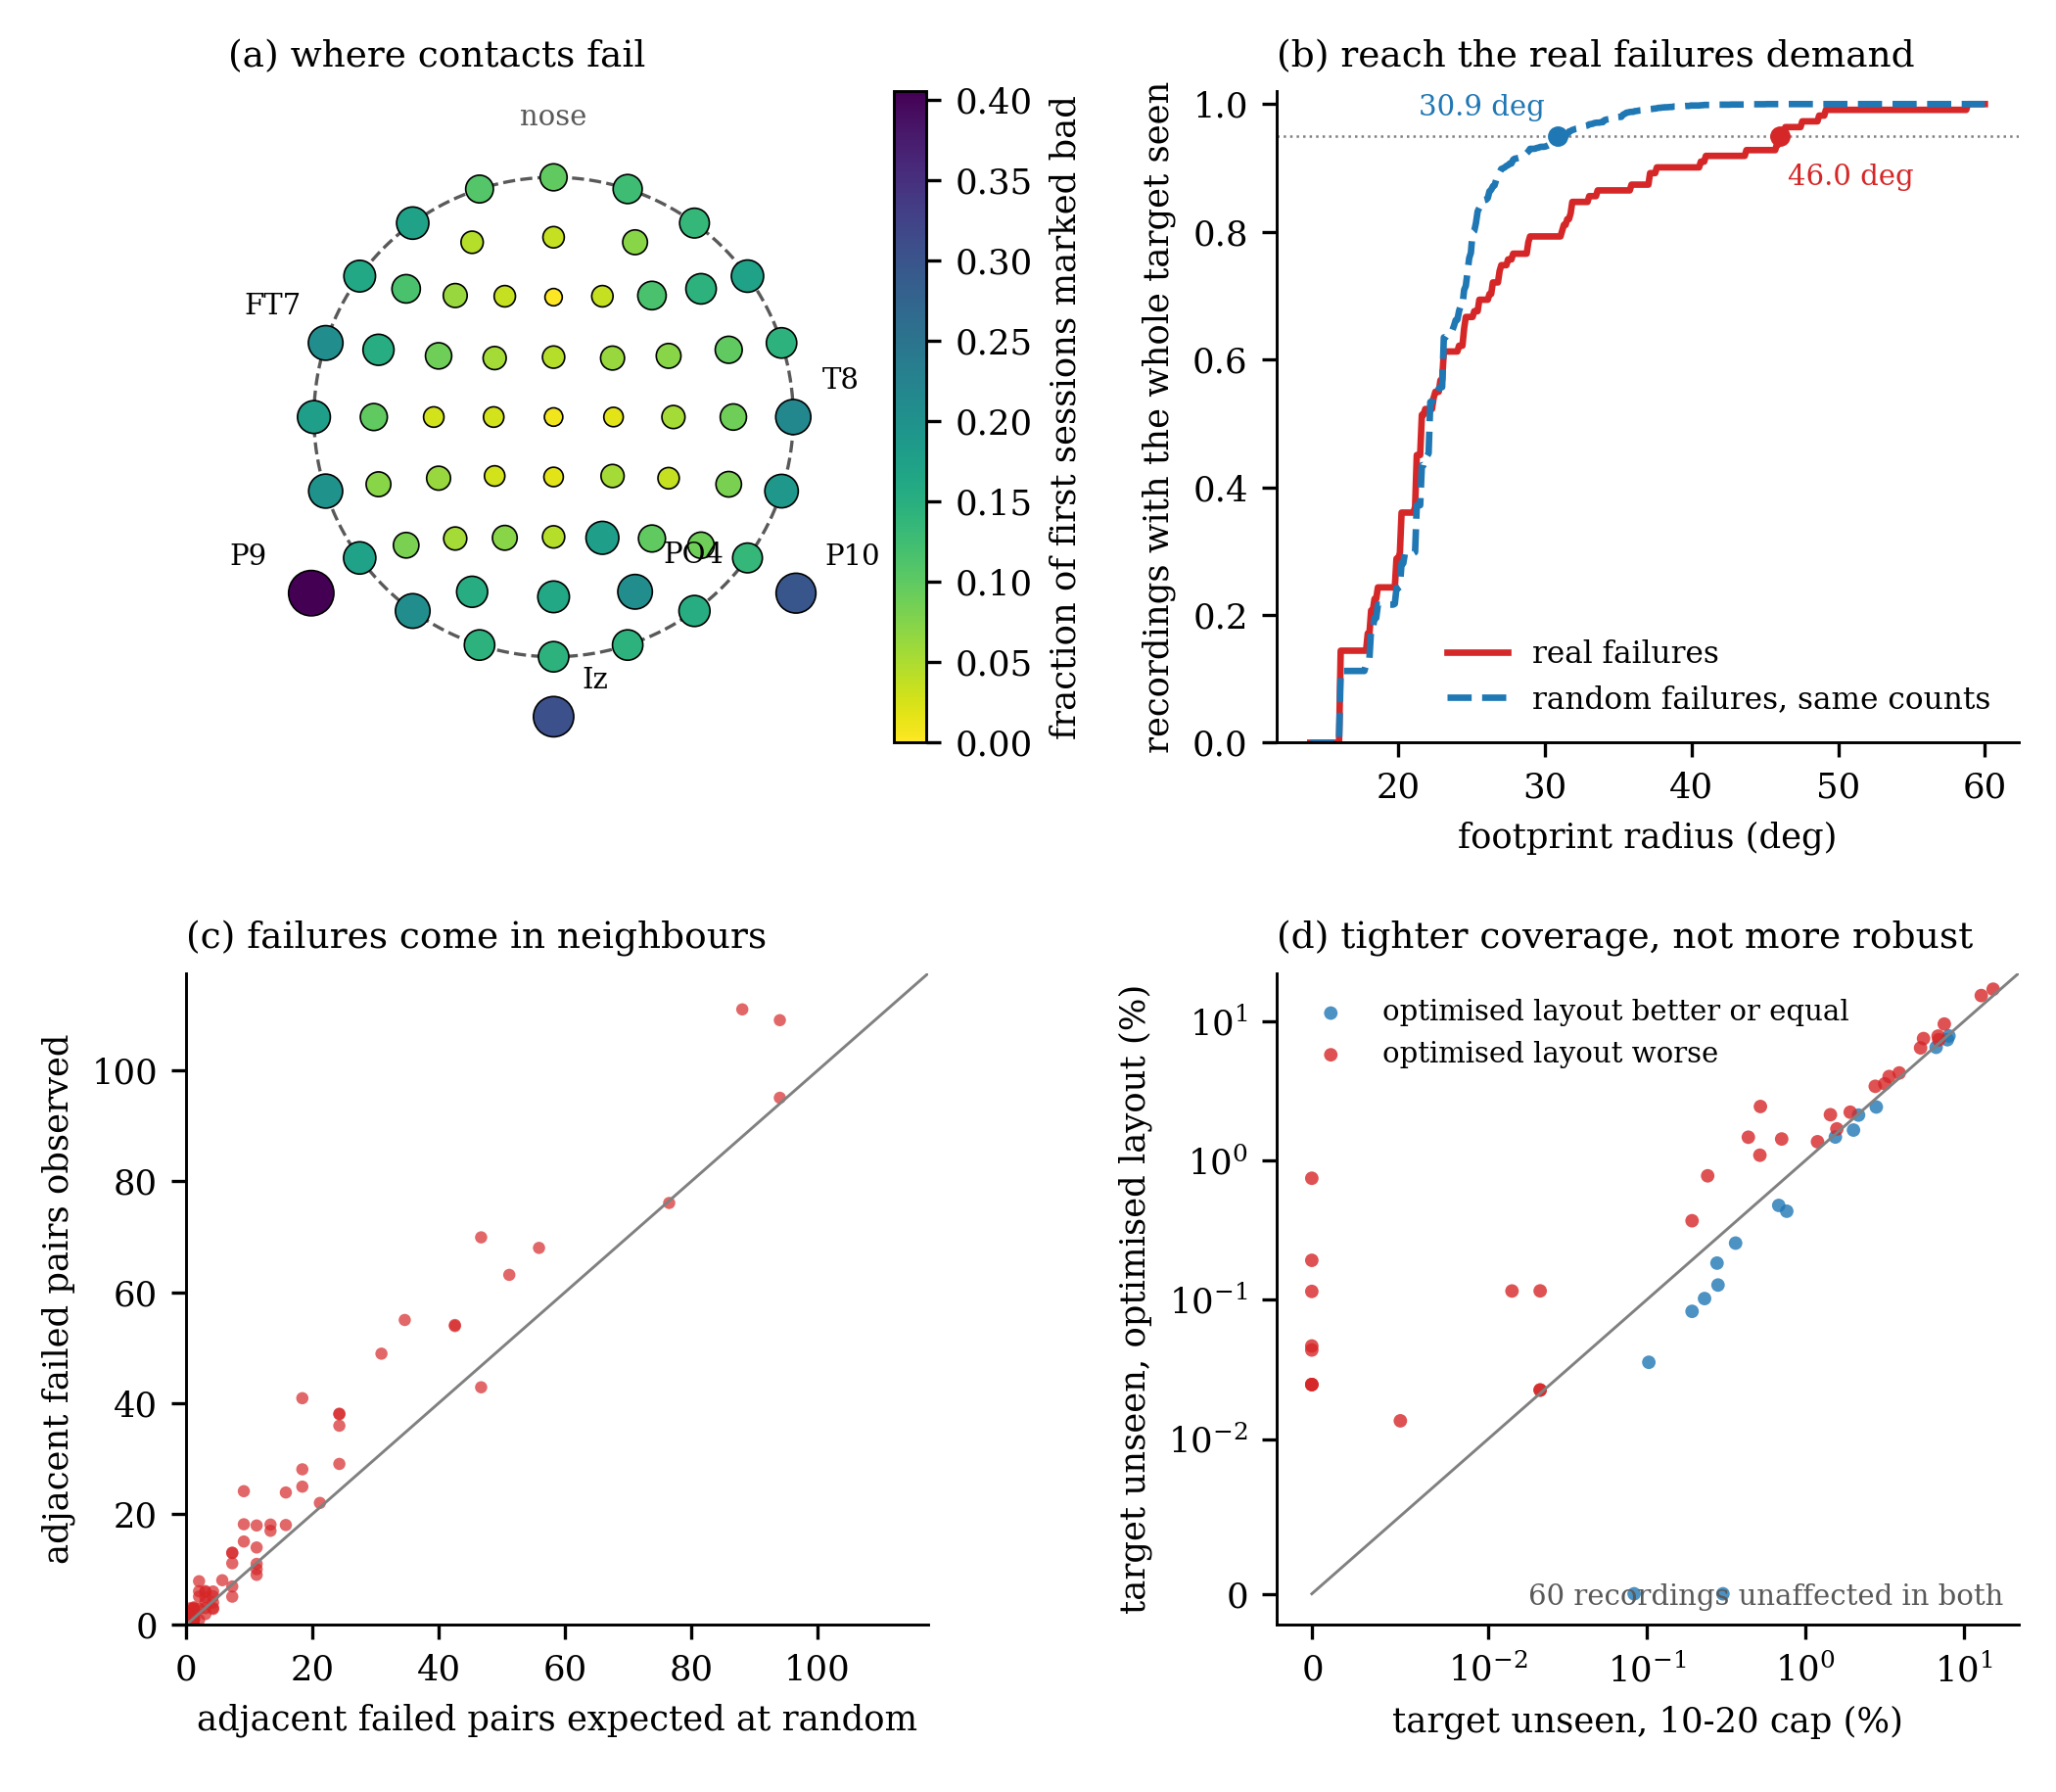
\includegraphics[width=\textwidth]{fig_eeg.png}
\caption{Real contact failures on the 64-channel cap, first sessions.
(a) Fraction of recordings in which each channel was marked bad. (b) Share of
recordings in which the survivors see all of $T$, against cap radius, for the
real failure sets and for random sets of the same sizes. (c) Adjacent failed
pairs, observed against the random expectation, one point per recording. (d)
Target unseen at $23.5^\circ$ by the standard cap and by the layout optimised
for 2-fold coverage, under the same real failures.}
\label{fig:eeg}
\end{figure}

\section{Does redundancy predict how well a lost channel is rebuilt?}\label{sec:signal}

Coverage is a statement about footprints, and a footprint is a model. The
test of whether it corresponds to anything physical is the signal. If a
channel is lost, its signal can be estimated from the channels that remain,
and the estimate should be better where the loss left more redundancy
behind. We fixed the plan for this test before any signal was loaded (Methods).
Every good channel of every recording was removed in turn and rebuilt from
all other good channels by spherical-spline interpolation~\cite{Perrin1989},
and the rebuild was scored by the Fisher-transformed correlation $z$ between
the true and rebuilt signal over four minutes. That gave \sigRows{} rebuilds
in \sigRec{} recordings, with median correlation \sigMedianR{}. One
second-session file of the \nRec{} published recordings contains no epochs and
could not be used.

\subsection*{Pre-specified tests}
The primary test is a natural experiment inside each channel. A channel's
position never changes, and what varies from recording to recording is which
of its neighbours failed, and hence its redundancy depth $\lambda$. Across the
first-session recordings, the Spearman correlation between $\lambda$ and $z$
was positive for all \sigPPos{} channels (median \sigPRho,
$p=\sigPP$). Private territory worked in the opposite direction, as specified
(\sigSoneNeg{} of \sigSoneCh{} channels negative, median $\sigSoneRho$,
$p=\sigSoneP$). Across channels within a recording, $\lambda$ still predicted
$z$ given the distance $d_1$ to the nearest survivor (median partial
correlation \sigStwoRho, positive in \sigStwoPos{} of \sigStwoRec{} recordings,
$p=\sigStwoP$). In the second sessions the primary test replicated (median
\sigSthreeRho, \sigSthreePos{} of \sigSthreeCh{} channels positive,
$p=\sigSthreeP$). All four pre-specified tests came out in the planned
direction.

\subsection*{What the result can and cannot say (exploratory)}
Three analyses written after these tests decide how to read them.

First, the within-channel design does not control for the recording. A
recording with many failed channels gives all of its channels a low $\lambda$,
and if such recordings are also noisier, every rebuild in them is worse,
with no local effect at all. With $z$ centred within each recording, the
within-channel correlation with $\lambda$ falls from \xwLamRho{} to
\xcLamRho{} but stays positive in \xcLamPos{} of \xcLamCh{} channels
($p=\xcLamP$; second sessions \xdLamRho, $p=\xdLamP$). Local redundancy is
real, and it predicts how well a lost channel can be rebuilt.

Second, by Proposition~\ref{prop:pairwise}, $\lambda$ is a sum over survivors
of a function of each survivor's distance. On all \sigRows{} rows it equals
$\sum_j K_\theta(\gamma_{cj})$ to within \lamDev{}, which is the sampling error
of the footprint areas. It is a geometric quantity. A purely metric
predictor, the mean distance to the three nearest survivors, does at least
as well within channel (median \xcDthreeRho{} with $z$ centred, $p=\xcDthreeP$),
and given those three distances, what $\lambda$ adds shrinks to a median of
\xcLamGivenDthreeRho{} (positive in \xcLamGivenDthreePos{} of
\xcLamGivenDthreeCh{} channels, $p=\xcLamGivenDthreeP$).

Third, prediction out of sample. With $z$ centred within recording, the six
nearest distances explain $R^2=\cvzMtwo$ under leave-one-subject-out
cross-validation (held-out second sessions \tezMtwo). Adding $\lambda$ and the
non-additive private territory $\pi$ changes $R^2$ by at most
\topoGainBound{} in either evaluation, with or without the channel site in
the model. The channel site itself adds \siteGain{}
(Fig.~\ref{fig:signal}b). So redundancy predicts how well a lost channel is
rebuilt, but the part of it that predicts is carried by distances. The
topology of the surviving coverage adds nothing measurable here.

\begin{figure}[t]
\centering
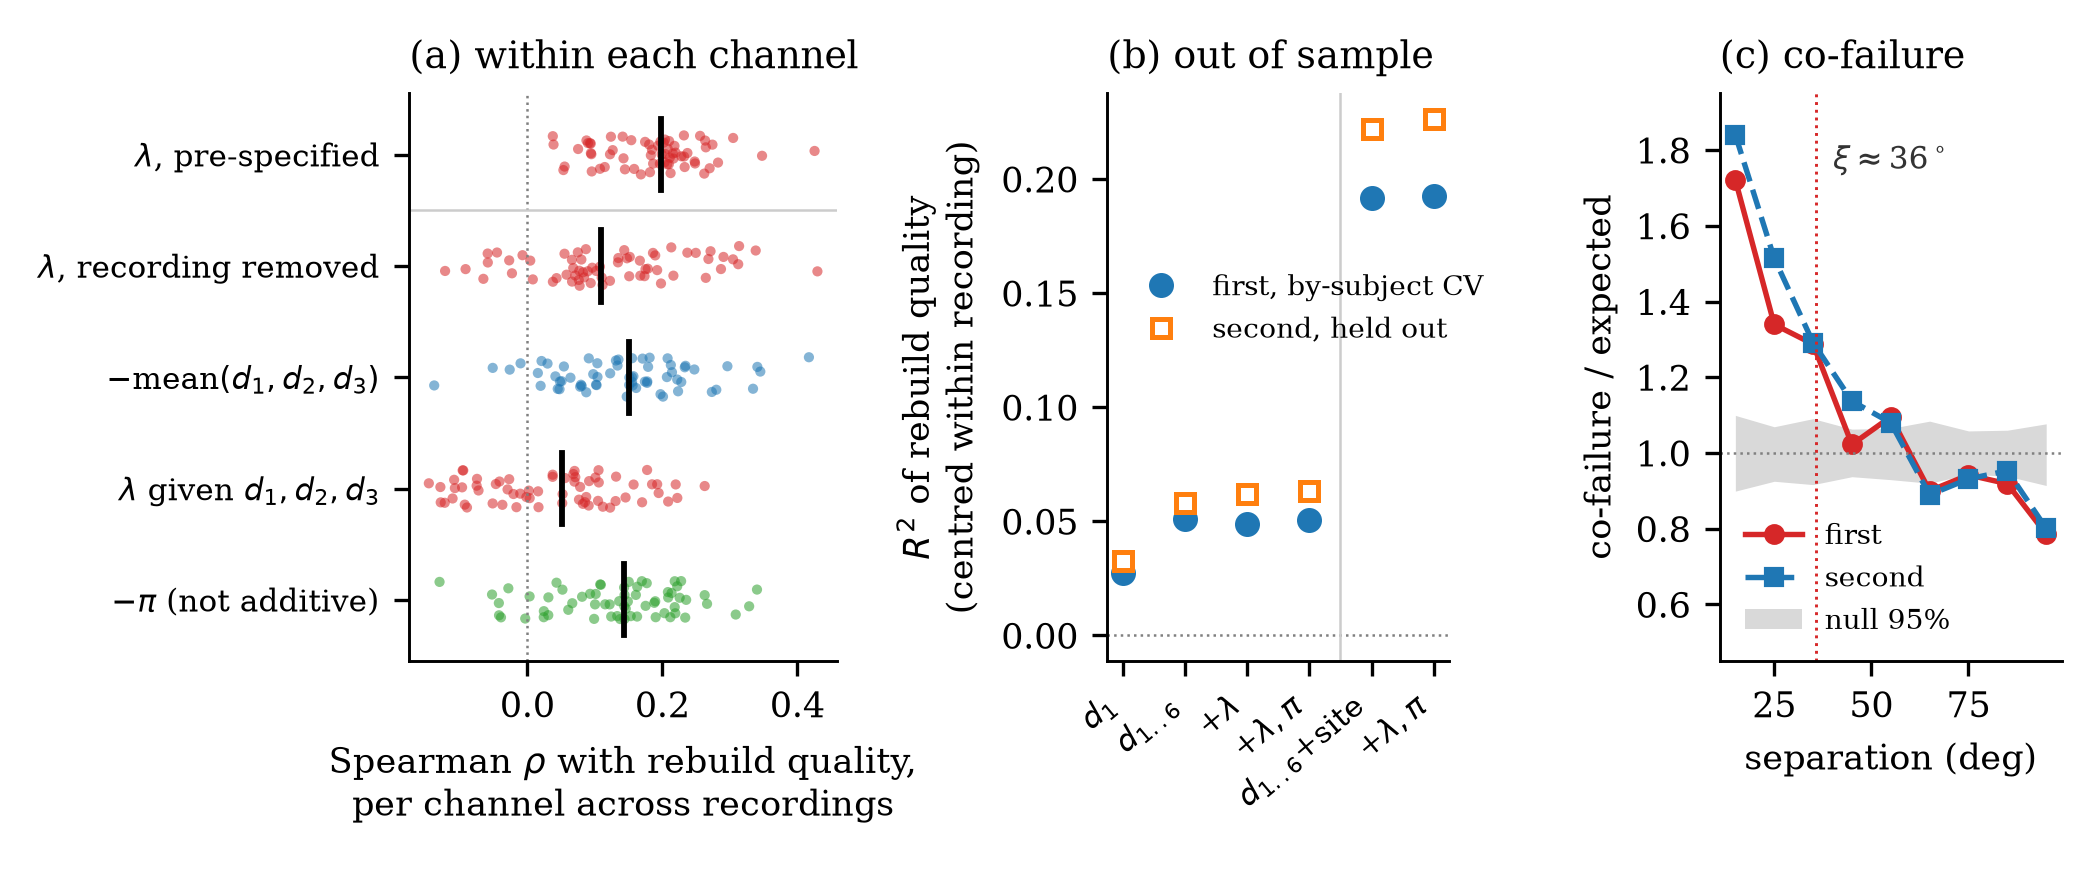
\includegraphics[width=\textwidth]{fig_signal.png}
\caption{(a) Within-channel Spearman correlation between each predictor and
rebuild quality, one point per channel, first sessions, with the median
marked. The top row is the pre-specified test. Those below are exploratory,
with rebuild quality centred within each recording. (b) Out-of-sample $R^2$ of
rebuild quality centred within recording, for nested models: the nearest
distance; the six nearest distances; with $\lambda$; with $\lambda$ and $\pi$;
the six distances with the channel site; and with $\lambda$ and $\pi$ added to
that. (c) Co-failure of channel pairs against their angular separation,
observed over expected under a null that keeps every recording's failure count
and every channel's failure rate, with the 95\% range of that null (first
sessions) and the correlation length $\xi$ at which the excess falls to $1/e$.}
\label{fig:signal}
\end{figure}


\section{Discussion}\label{sec:discussion}

\subsection*{What the evidence supports}
The certificate is exact where its hypothesis holds: on the scalp it
reproduced the exact topology of the $k$-fold region for every real failure
pattern. On a folded cortex, where geodesic footprints are not convex, it can
miss a hole, so it has to be checked against a direct computation there. It
gives the shape of the $k$-fold region and not whether that region contains
the target. Real failures are clustered, recur
within a subject and concentrate at the rim, and they are correlated in space beyond what each channel's failure rate
explains, over about \xiOne$^\circ$. Redundancy
predicts how well a lost channel is rebuilt, but through distances. What has
not been shown is that the topology of the coverage changes an outcome that
distances do not already predict, and that is the claim a physical or
clinical reader would need. This paper does not make it.

\subsection*{What would change this picture}
Four results would. The first is clinical. Whether the certified coverage of
the resected territory predicts seizure freedom after epilepsy surgery can
be tested on open intracranial recordings that carry electrode coordinates,
resection information and surgical outcome, such as OpenNeuro
ds003029~\cite{Li2021}. The protocol reconstructs each patient's pial
surface, places that patient's own contacts, computes the covering radius and
certified level over the resected region, and tests them against outcome, all
under a plan fixed before any outcome label is read. Incomplete resection of the seizure onset zone has been reported not to
predict outcome~\cite{Gascoigne2024}, so the result could go
either way, and a null would end the clinical claim. Before any such dataset
is used, its data descriptor and the independent studies that reuse it should
be checked, to make sure the released version is the one that produced
published results.

The second is a law for correlated failure. The required reach at 95\% is
set by the largest region that the failures empty. A theory giving that reach
from a measured failure correlation length, in the manner of correlated site
removal on a covering, would predict the reach before the data arrive. It
would have to be confirmed on an independent dataset with curated channel
status. The correlation length measured here is the input such a theory needs,
but it is not yet the theory. Its interval is wide, and it comes from one
cap, one laboratory and one curation pipeline.

The third is a design that wins out of sample. The layout that lost was
optimised for tight double coverage. A layout optimised against the loss of
adjacent pairs at the rim, chosen on one dataset and scored on another, would
turn the negative result of Section~\ref{sec:failures} into a positive one.

The fourth is mathematical. Two problems are open: a combinatorial
condition, checkable on $N$ and a description of $T$, that forces
$T\subseteq R_k$; and a stability theorem for
the two-parameter module indexed by footprint radius and
multiplicity~\cite{CarlssonZomorodian2009} under perturbation and deletion of
contacts, extending the one-parameter bounds~\cite{CohenSteiner2007} measured
in the supplementary code.


\section{Methods}\label{sec:methods}

\subsection*{Footprints and targets}
Scalp positions are the 64 BioSemi positions of MNE-Python's standard
montage~\cite{Gramfort2013} as unit vectors, with Cz at the pole and the
Fpz--T7--Oz--T8 circumference at colatitude $92^\circ$. Areas on the sphere are
measured on a Fibonacci lattice of $4\times10^6$ points, of which about
$2.07\times10^6$ fall in $T$. The cortical surface is the left pial surface of
colin27 from the FieldTrip toolbox, 175\,409 vertices, with every edge in two
triangles and Euler characteristic~2. Geodesic distances are Dijkstra
distances on the mesh edges, and a triangle belongs to a footprint when all
three of its vertices do.

\subsection*{Nerves and Betti numbers}
For caps of radius below $30^\circ$, any subfamily whose triples meet lies in
an open hemisphere about each of its centres, and the gnomonic chart maps it to
planar convex sets, so Helly's theorem makes the nerve the flag completion of
its triangles. A triple of caps meets when the minimal enclosing cap of its
centres has radius below $\theta$. Betti numbers $b_0,b_1$ of $\Delta_k(N)$
are computed over GF(2) from its 2-skeleton. The exact reference for $R_k$ on
the sphere is computed from the arrangement of the boundary circles, with no
nerve involved; the raster reference counts components and holes of
$\{m\ge k\}$ in a stereographic chart of $4000^2$ pixels.

\subsection*{Statistics}
All tests are one-sided in the direction stated in the plans, with
$\alpha=0.05$, and use the Wilcoxon signed-rank test~\cite{Wilcoxon1945} or
Monte Carlo tests with $p=(1+\#\{\text{null}\ge\text{observed}\})/(1+M)$.
Seeds are fixed in the code. The plans for the failure analysis and the
signal-level test are the docstrings of \texttt{run\_eeg\_failures.py} and
\texttt{run\_signal\_rebuild.py}, committed before the respective outcomes
were computed. Every analysis labelled exploratory was written afterwards.

\subsection*{Signal-level test}
The curated epochs of ds003775 v1.2.1 (band-pass 1--45\,Hz, average
reference, 60 epochs of 4\,s at 1024\,Hz per recording) were fetched by S3
object version and checked against the size and MD5 of each file's
git-annex key. Channels the curators marked bad had been interpolated by
their pipeline and were used neither as targets nor as inputs. In each
recording, each good channel $c$ was removed and rebuilt from all other good
channels by spherical-spline interpolation~\cite{Perrin1989} (stiffness 4, 50
Legendre terms, regularisation $10^{-5}$, the MNE-Python
defaults~\cite{Gramfort2013}). Rebuild quality is the Fisher transform
$z=\operatorname{artanh} r$ of the correlation $r$ between the true and rebuilt
signal over all 240\,s. For the survivors $S$ and the primary radius
$23.5^\circ$ we recorded $\lambda(c,S)$, $\pi(c,S)$, the number of survivors
within $23.5^\circ$ and the angle $d_1$ to the nearest survivor. The
pre-specified primary test (P) takes, for each channel that is a good target
in at least 10 first-session recordings with at least 3 distinct values of
$\lambda$, the Spearman correlation between $\lambda$ and $z$ across those
recordings, and tests with a one-sided Wilcoxon signed-rank test over channels
that these correlations are positive. A channel's position never changes, so
what varies between recordings is which of its neighbours failed: a natural
experiment inside each channel. Test S1 is the same with $\pi$ in the negative
direction; S2 is the partial Spearman correlation of $z$ with $\lambda$ given
$d_1$ across channels within each first-session recording, one-sided over
recordings; S3 repeats P on the second sessions.

\subsection*{Exploratory analyses}
(i) Proposition~\ref{prop:pairwise} was checked on every row by evaluating
$K_\theta$ by quadrature. (ii) The within-channel test was repeated with
metric predictors and with partial correlations given the nearest one and
three distances. (iii) Rebuild quality, centred within each recording to
remove every recording-level effect, was predicted by nested least-squares
models: $d_1$ and $d_1^2$ (M1); the six nearest distances and their squares
(M2); M2 with $\lambda,\lambda^2$ (M3); M3 with $\pi$ and $\mathbf 1[\pi>0]$
(M4); M2 with 63 channel indicators (M5); M5 with $\lambda,\pi$ (M6). Models
were scored by leave-one-subject-out cross-validated $R^2$ on the first
sessions, and, fitted on all first sessions, on the second sessions as a held
out set. (iv) The clustering statistics were compared with a null that keeps
each recording's number of failures and each channel's number of failures,
sampled by curveball swaps~\cite{Strona2014} (\mgNull{} null cohorts, 1000
swaps apart after a burn-in of 20\,000), and with the uniform null of the plan.
(v) Pair correlation of failure: for channel pairs binned by angular
separation in $10^\circ$ bins, the number of recordings in which both failed,
divided by its mean over the same null cohorts. The correlation length is the
separation at which the excess over one falls to $1/e$ of its value in the
first occupied bin, interpolated linearly between bin centres, with a 95\%
interval from 2000 bootstrap resamples of recordings.


\section*{Data availability}
OpenNeuro ds003775 v1.2.1 (doi:10.18112/openneuro.ds003775.v1.2.1, CC0). The
cleaned-epoch files are fetched by their S3 object versions, and the version
ids are recorded with each file's size and MD5 in
\texttt{data/ds003775\_epochs\_manifest.tsv}, since later versions of the dataset
dropped them. The colin27 surface is derived from FieldTrip commit
\texttt{8e2307d}. No patient data are used.

\section*{Code availability}
All code, the analysis plans and every result file quoted here are at
\url{https://github.com/creelie/kshadow-coverage}. Every number in this
manuscript is a macro generated from those result files by
\texttt{make\_paper\_numbers.py}.

\section*{Author contributions}
[To be completed by the authors.]

\section*{Competing interests}
The authors declare no competing interests.

\bibliographystyle{amsplain}
\bibliography{refs}

\end{document}
